\section{Vertiefungsprojekt: MiniMax TicTacToe}

Um den MiniMax-Algorithmus besser zu verstehen, wurde der Algorithmus f�r ein TicTacToe-Spiel in Java implementiert. Diese Implementierung basiert auf einem Online-Artikel von GeeksForGeeks\cite{minimax-online}.

\begin{figure}[H]
    \centering
    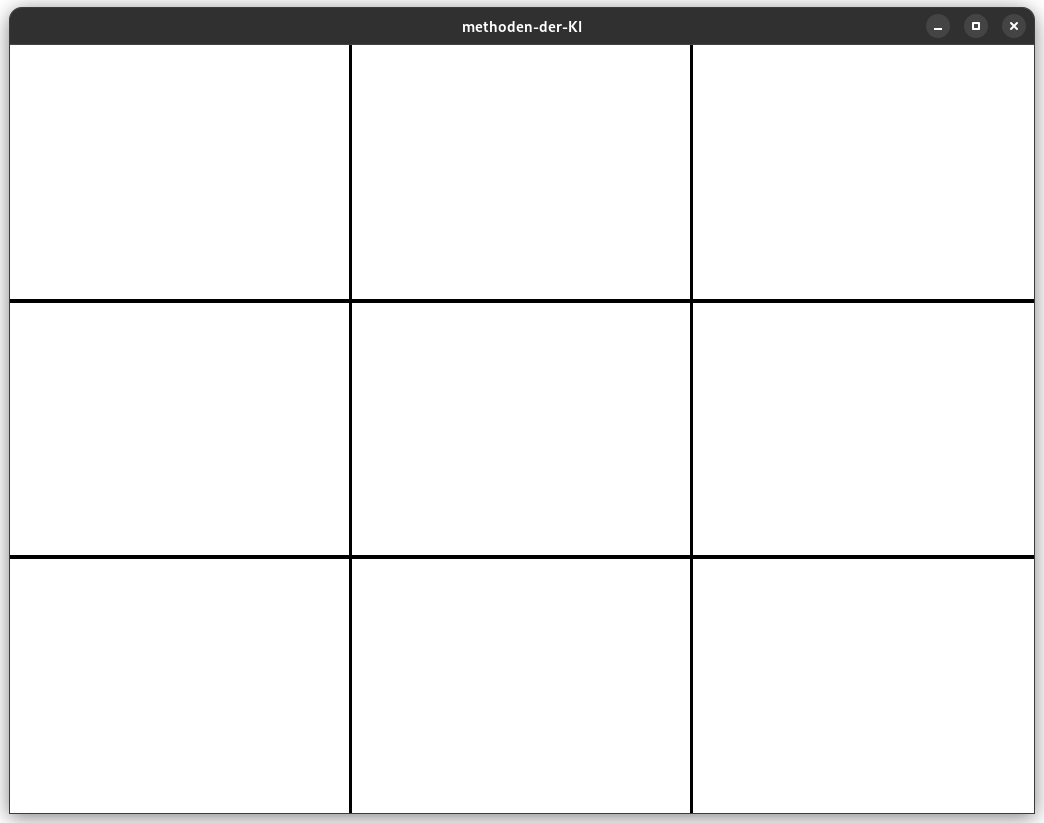
\includegraphics[width=0.6\textwidth]{figures/kap4/impl-minmax.png}
    \caption{Das leere Tic-Tac-Toe-Raster}
    \label{fig:empty-tictactoe}
\end{figure}

Das Spiel beginnt entweder mit einem leeren Raster oder mit einem Kreis in der unteren linken Ecke. Dies liegt daran, dass zu Beginn des Spiels eine Wahrscheinlichkeit von 50\% besteht, dass die KI den ersten Zug macht. Dieser Zug ist normalerweise die untere linke Ecke (was, wie sich herausstellt, der beste Zug ist, wenn man zuerst beginnt).

In dieser Implementierung spielt der Spieler immer als Kreuz und die KI als Kreis. Um einen Zug zu machen, klicken Sie auf die Zelle, die Sie mit einem Kreuz f�llen m�chten. Sobald jemand gewonnen hat (der menschliche Spieler kann in diesem Fall jedoch nicht gewinnen) oder keine leeren Felder mehr im Raster vorhanden sind, wird ``Game Over'' angezeigt.

\begin{figure}[H]
    \centering
    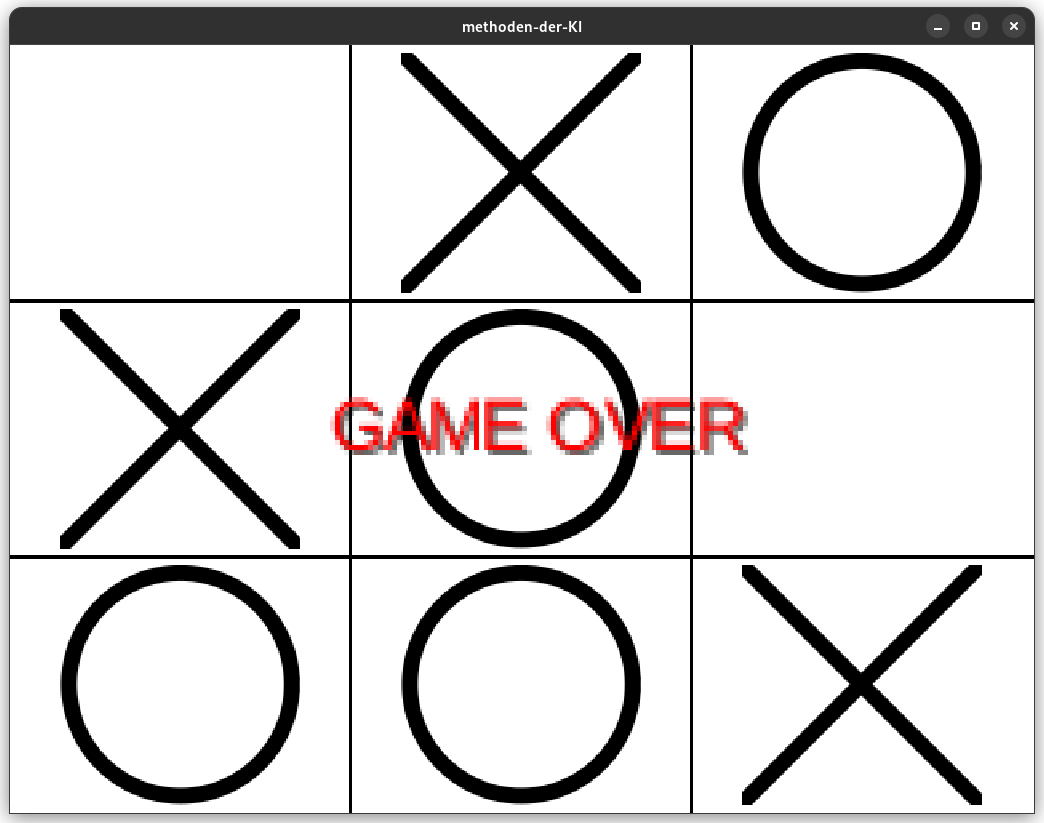
\includegraphics[width=0.7\textwidth]{figures/kap4/ttt-gameover.png}
    \caption{Game over!}
    \label{fig:ttt-gameover}
\end{figure}

Die Tastensteuerungen wie folgt:
\begin{itemize}
    \item \textbf{Leertaste:} Setzt das Spiel zur�ck. 
    \item \textbf{Escape-Taste:} Geht zur�ck zum Start-Screen.
\end{itemize}

Der relevante Code f�r das Programm befindet sich in den folgenden Packages (Implementierungscode befindet sich im ``core'' Verzeichnis):
\begin{itemize}
    \item \textbf{de.augsburg.hs.methoden.ki.screens.minmax:} Der Code f�r den MiniMax-Screen.
    \item \textbf{de.augsburg.hs.methoden.ki.algorithms.minimax} Klassen f�r die Implementierung des MiniMax-Algorithmus.
    \item \textbf{de.augsburg.hs.methoden.ki.actors.minimax:} Klassen f�r das Kreuz und den Kreis.
\end{itemize}